\documentclass[a5paper,twoside,12pt]{report}

%%%%%%%%%% Packages %%%%%%%%%%
\usepackage[outer=2cm, inner=2cm]{geometry}
\usepackage{fancyhdr}
\usepackage{microtype}
\usepackage{graphicx}
\usepackage{wrapfig}
\usepackage{enumitem}
\usepackage{amsmath}
\usepackage[utf8x]{inputenc}
\usepackage[english]{babel} 
\usepackage{epigraph}
\usepackage{lmodern}
\usepackage{afterpage}
\usepackage{nonumonpart}
\usepackage{titlesec}
\usepackage{microtype}
\usepackage{titling} 
\usepackage[T1]{fontenc}
\usepackage{bold-extra}
\makeindex

\newlength\longest
\setlength{\marginparwidth}{0pt}

\titleformat{\section}[wrap]
{\normalfont\bfseries}
{\thesection.}{0.5em}{}
\titlespacing{\section}{12pc}{1.5ex plus .1ex minus .2ex}{1pc}
\pagestyle{fancy}
\fancyhf{}
\fancyhead[LE,RO]{\thepage}
\fancyhead[LO]{\leftmark}
\fancyhead[RE]{The Inferno Adventures}
\fancypagestyle{plain}{%  the preset of fancyhdr 
  \fancyhf{} % clear all header and footer fields
  \fancyhead[LE,RO]{\thepage}
  \fancyhead[LO]{\leftmark}
  \fancyhead[RE]{The Inferno Adventures}}

\begin{document}
\pagenumbering{gobble} 

%%%%%%%%%% Pretitle %%%%%%%%%%
\title{%
  Adventures in Trying the Inferno Operating System
}
\date{}
\author{}
\maketitle

%%%%%%%%%% EMPTY PAGE %%%%%%%%%% 
\thispagestyle{empty}
  \mbox{}
  \newpage

%%%%%%%%%% Posttitle %%%%%%%%%% 
\title{%
  Adventures in Trying the Inferno Operating System \\
  \begin{center}\textit{Observations and Notes}\end{center}
  \author{By Marvin Johanning}
}
\maketitle

%%%%%%%%%% Copyright and Impressum %%%%%%%%%%
\thispagestyle{empty}
\noindent\textsc{\underline{Text}}: © Copyright 2020 Marvin Johanning

\noindent\textsc{\underline{Cover design}}: © Copyright 2020 Marvin Johanning

\vspace{8mm}\noindent\textbf{\underline{Copyright (C) 2020 Marvin Johanning.}}

\noindent© 2020 by Marvin Johanning\\``Adventures in Trying the Inferno Operating System'' by Marvin Johanning is licensed under CC BY-NC-SA 4.0. To view a copy of this license, visit https://creativecommons.org\allowbreak/licenses/by-nc-sa/4.0.

\vspace{20mm}\noindent\textsc{Publishing}: \\
Marvin Johanning\\
Salzufler Str. 66\\
33719 Bielefeld\\
info@marvinjohanning.de

\vspace{25mm}\noindent\textsc{Printing}: epubli – ein Service der neopubli GmbH, Berlin
\newpage

%%%%%%%%%% Introductory quote %%%%%%%%%%
\clearpage
\thispagestyle{empty}
\null\vfill
\settowidth\longest{\huge\itshape We have persistent objects,}
\begin{center}
\parbox{\longest}{%
  \raggedright{\huge\itshape%
    We have persistent objects, \\they're called files. \par\bigskip
  }
  \raggedleft\Large\MakeUppercase{Ken Thompson}\par%
}
\vfill\vfill
\clearpage\newpage
\end{center}
\newpage

\tableofcontents
\pagebreak

%%%%%%%%%% Introduction %%%%%%%%%%
\pagenumbering{roman}
\chapter*{Introduction}
  \markboth{Introduction}{Introduction}
  \addcontentsline{toc}{chapter}{Introduction}
In the following document you will be presented with some information regarding the Inferno operating system created by Bell Labs in the mid 1990s. Its name and somewhat mysterious aura led me to write it in a style akin to the one that can be seen in older books, such as those from the early 20th or late 19th centuries. This applies to both the chapter headings, as well as the text itself.

I believe that this may also make reading it somewhat more enjoyable than the otherwise rather dryly written literature available on this subject and perhaps help those who are interested in this operating system — and that may possibly not know much about Linux itself either — can have an interestingly written introduction.

It is however to be noted that this is not meant to be a complete introduction to the operating system and its underlying structure; it is merely intended to be a quick overview of the operating system, how to install it and what you can do with it.

I highly encourage to to critisise my work — this is, obviously, without having to result to petty insults and the like — and send me an email with your feedback. It is not unlikely that I have made a mistake — or perhaps even several — over the course of this document and I always like to be corrected if there are factual, grammatical or spelling errors.

This work is licensed under a Creative Commons license, which means you are allowed to share it with others free of charge and I do encourage you to do so; you should never have to pay for this document in a digital format and I would like you to report any such occurences to me, since commercial distribution is strictly prohibited by the license and those who make a profit from it are in violation of it. Physical copies can be obtained solely from me, at least commercially. 

\newpage

%%%%%%%%%% About %%%%%%%%%%
\chapter*{About me}
  \markboth{About me}{About me}
  \addcontentsline{toc}{chapter}{About me}

  My name is Marvin Johanning, I'm twenty-one years old and currently reside in a city many deem to not exist — which, obviously, is untrue for I \textit{do} live here and surely I am real. I like writing things, even though, perhaps, I am not great at it; yet I enjoy doing so and only through practice can you improve, which is why I write as much as possible as frequently as I can.

  I have recently switched from writing in LibreOffice to \LaTeX, as LibreOffice has proven itself to be headache-inducing when working with large amounts of text which you wish to reformat at a later date. 

  I tend to write about things relating to languages — be it real or programming languages —, computers and, though rarely, politics. All of these can be found on my website. My biggest writing project to-date is \textit{The Intricacies of Ancient Egyptian Hieroglyphics} (ISBN: 978-3-752952-49-0), which incidentally was what lead me to use \LaTeX, which is still to be done; information regarding it can, too, be found on my website.
  \newpage


%%%%%%%%%% Empty page %%%%%%%%%%
\pagenumbering{gobble}
\thispagestyle{empty}
  \mbox{}
  \newpage

%%%%%%%%%% Beginning of text itself %%%%%%%%%%
\pagenumbering{arabic}
\part*{Book I}
  \markboth{Book I}{Book I}
  \addcontentsline{toc}{part}{Book I}
  \newpage

\thispagestyle{empty}
  \mbox{}
  \newpage

\chapter*{From the Deepest Depths of Hell}
  \markboth{From the Deepest Depths of Hell}{From the Deepest Depths of Hell}
  \addcontentsline{toc}{chapter}{From the Deepest Depths of Hell}

\epigraph{``Long is the way and hard, that out of Hell leads up to light.''}{\textit{John Milton\\Paradise Lost, Book II}}

I must admit, it was largely the rather intriguing name of this operating system that made me want to know more about it and do more research on it. I had come across it on one of my quite common internet \textit{trips} wherein I simply hop from one hyperlink to the next, trying to discover something interesting — or, perhaps more accurately, something obscure. 
Frequently these \textit{trips} end unsatisfactorily; yet this time, luck seems to have been on my side, for I was finally able to uncover something interesting — why, even mysterious. I am of course speaking of the \textit{Inferno operating system} created by the renowned Bell Labs in 1996. 

They had previously worked on \textit{Plan 9 from Bell Labs} — why they felt the need to add the ``from Bell Labs'' portion is, unfortunately, beyond me — which, just as Inferno, has largely fallen into obscurity. It is now just to be found in the dark and long forgotten and abandoned corners of the web that seem to be frozen in time, containing information and discussions from days long past; that are held aloft simply by someone continuing to pay for server bills. It's a pity, really, how large amounts of information can simply vanish from the world by someone — perhaps quite literally — pulling the plug.

Plan 9 — as I will be calling it henceforth, ignoring the \textit{from Bell Labs} portion of its name, for I trust you will know that I am indeed referring to the operating system and not the movie — was actually what I had found prior to Inferno.

I am unsure of the precise circumstances that let me to its discovery, but I distinctly remember discovering a page filled with interesting documents on a wide range of topics which can be reached under the following address: \texttt{http://doc.cat-v.org/}. 
This fascinating archive of old documents contains a myriad of interesting tidbits on both Plan 9 and Inferno — and other topics as well. 

I thus decided to start reading some of the documents available on Plan 9 and was quickly intrigued — for seeing an operating system whose creators are the same ones that created the beauty that is UNIX was truly remarkable; why had I not heard of it previously?

Yet to my utter dismay, it was quickly revealed that it seems to have been long forgotten and abandoned — but a mere relic of the past — and that one can count its user base on two hands; and while there appears to remain a small number of people that continue using it, its ultimate failure was being unable to prove much better than what it strove to replace — UNIX itself.

For they realised their old operating system had become \textit{too} old, even by the standards of the mid-1980s. They wished to create a system — from scratch — that would encompass these new-fangled ideas, such as graphical user interfaces; a system that did not have these features hapharzardly stiched on — as a surgeon would try to fix a severly wounded fellow — but one that was built with them in mind; a system that would abide by UNIX' philosophy of everything being a file, but one that was more adapt to modern — at least, for the time — standards.

But alas, as the passage of time has revealed, their efforts have been in vain; for ask any fellow, even those who are learned and know of computers, and chances are high he will not know of their failed efforts to create a superior UNIX.

Yet this is not a tale of Plan 9, it is one of its successor Inferno. Having learnt from their former mistakes with Plan 9, they strove to create a superior Plan 9; one that would be used in network environments; one that was portable and lightweight and could easily run on a myriad of different types of machine.
Yet tragically, even Inferno seems to have gone under — perhaps even into hell itself.

But fret not! While abandoned by Bell Labs long ago — what vile traitors they are! —, it has since been acquired by an American company, who have released the latest version in 2015. Let us unveil this long forgotten gem. \newpage

\chapter*{Resurrecting the Devil}
  \markboth{Resurrecting the Devil}{Resurrecting the Devil}
  \addcontentsline{toc}{chapter}{Resurrecting the Devil}

  \epigraph{``Soon you will be where your own eyes will see the source and cause and give you their own answer to the mystery.''}{\textit{Dante Alighieri\\The Divine Comendy, Inferno}}

  The first question that arises is whence one can obtain a copy of this operating system and it seems the official source code is currently available on GitBucket; but one may also download it from the current maintainers' website: http://www.vitanuova.com/index.html. This appearance of this website, too, reminds one of those long forgotten sites filled with flashing GIFs and strangely formatted text from the late 1990s or early 2000s. Yet it appears that it has yet to be abandoned — why, there seem to exist discussion forums dedicated to Inferno still! What a site to behold they are; and though posted on only occasionally, it is a pleasure to see discussions being conducted about Inferno — there may be hope still! But let us continue with our journey down into the depths of hell.

  Obtaining the latest version of this operating system is a task swiftly completely; indeed, it is a mere 70 megabyte large archive — 'tis truly devilish sorcery worthy of the name  ``Inferno''.

  Yet already we stumble across something strange; something unusual; something you shan't see with an operating system of current times — why are there different downloads for different operating systems. Surely, you cannot imply it is to be run ontop of another operating system? Why yes, you can.

  Indeed, something I had negelected to mention previously was the fact Inferno is no ordinary operating system — no, it is meant to be installed ontop of the one already running on one's machine; and whilst it is indeed possible to install it onto bare hardware, only a madman would do such a thing. Really, its main intent was to be a complentary system to Plan 9 and one was meant to install it ontop of Plan 9 to have a more complete experience.

  Thus choose wisely; do not download the wrong archive, for it may not work. As I am running Linux, I chose their archive meant to be used with Unix-like systems, of which Linux is one. It is, as previously mentioned, an archive and must thus be extracted, a task easily accomplished with Linux' helpful \texttt{tar} command; one must simply type \texttt{tar xf} followed by the name of the archive and it is extracted into its own directory.

  Upon entering the directory so thoughtfully created by the \texttt{tar} command, one is greeted by files upon files and folders upon folders. Indeed, it may be slightly disorienting — even offputting — to those uninitiated to Unix-like systems; but, as one is swift to notice, there are two helpful documents to guide us in our installation journey: a \texttt{README.md} and an \texttt{INSTALL} document. Therein you will find a lot of information that will be imperative for installing Inferno; thus, let us first take a look at the README.

  Inside the README one finds general information regarding the operating system, detailing its creators and purpose. Additionally it highlights what makes it so interesting — yet also similar to Unix: —

  \begin{quote}
    The use of a high-level language and virtual machine is sensible but mundane. The interesting thing is the
    system’s representation of services and resources. They are represented in a file-like name hiearchy.
    Programs access them using only the file operations open, read/write, and close. The ‘files’ may of course
    represent stored data, but may also be devices, network and protocol interfaces, dynamic data sources, and
    services.
  \end{quote}

  It is truly remarkable; a system whereon everything is a file — something that can readily be read and edited — is revolutionary and yet it is simple — why, even mundane! A mere child could think of it. It is, beyond any doubt, an elegant and ingenious idea.

  But withal, this helped but little in embarking onto our journey into Inferno; and whilst it was indeed interesting to be given some information regarding its background, we are none the wiser. Thus, let us read the INSTALL file, wherein we shall — hopefully — find our answers; and indeed we do!
  For therein we are presented with actual instructions, but as they may appear cryptic to those who have never — or perhaps only rarely — used a Unix-based operating system, I shall try to elaborate on their instructions; for they merely appear cryptic — or, perchance, even challenging — and are, in actuality, quaint and mundane.

  It is, however, to be noted that my instructions henceforth will work only on Linux x86; should you wish to be presented with instructions regarding other systems — systems whose name should not be spoken, for they are vicious and vile, forged somewhere far below hell itself; in a place Be\"{e}lzebub himself does not dare to enter — you may cease your reading here, for you may not find the information you desire. The following chapter is akin to a recipe from a cook book; hence follow the instructions with care, or your ``meal'' may turn out wretched, ugly and inedible.

  One must first define the \textit{root} of the installation; this may sound somewhat strange, yet in actuality one is simply required to aid Inferno in knowing where on your system it is located — it cannot know on its own and assumes it is located in \texttt{/usr/local/inferno}. Hence, should you not wish Inferno to be installed there, you must alter the \texttt{mkconfig} file; therein you can modify the \texttt{ROOT} variable to point to your Inferno directory.
  Yet withal, I would recommend simply using the directory Inferno wishes to be inside of by creating it using \texttt{sudo mkdir /usr/local/inferno} and thereafter copying the contents from the old directory to the new one by typing \texttt{sudo cp -r * /usr/local/inferno}; I have found this to be much more simple. You must then move into this directory by typing \texttt{cd /usr/local/inferno}.

  But be aware! Apart from the \texttt{ROOT} variable, there exist two others, namely \texttt{SYSHOST} and \texttt{OBJTYPE}; it is imperative to modify these so that they match your system, for otherwise your installation will fail — indeed, this is akin to letting a scoundrel wreak havoc on your system. Thus — this is, unless you are using one of the aforementioned systems whose names should never be mentioned, for they cause terror and fear far greater than that caused by the devil himself —, pay heed to the values of these two variables, for they ought to be set to \texttt{Linux} and \texttt{386} respectively. The latter should be modified to equal \texttt{arm} should your Linux installation be ARM-based, such as those running on the Raspberry Pi.

  Having completed this task, you will thence be able to execute \texttt{makemk.sh}, a shell script that will spawn the \texttt{mk} executable which shall thenceforth be used for building Inferno itself; a infernal tool for certain, yet one that shall prove invaluable.

  I implore you to act with as much care as you can permit henceforth, for the following commands utilise \texttt{sudo}; an almighty tool whose purpose is to allow you to be the lord of your system; a tool that grants you the permissions to do every conceivable thing on your machine; a tool that is a juxtaposition of both Good and Evil, for it imparts you with the power of achieving your every desire, but it may also destroy what you have created in an instant. Should your machine contain data you believe invaluable, I urge you create a copy of it elsewhere; in a place where Satan cannot touch it.

  Notwithstanding, it must be used, for our machine will not permit us to make changes without it; you may attempt to run \texttt{makemk.sh} without \texttt{sudo}, but you shall be given an error, as one may not make any changes to the system without having been having been granted the appropriate privileges.

  If you deem yourself to be prepared, execute \texttt{sudo ./make\\mk.sh} whereupon you may be presented with a number of warnings that can, however, be ignored; for if, after a few seconds, you are told that ``mk binary built successfully!'', everything has worked and a binary has been concocted and can thence be found inside \texttt{/usr/local/inferno/Linux/386/bin}.

  But alas, our machine is dim-witted, for running \texttt{mk} does not yield anything; nay, it appears the command does not exist — which is undoubtebly wrong, for its existance can be ascertained by looking at the aforementioned directory. So what is one to do? The machine needs to be told where to find it — and the binaries that shall be brought into existance soon —, which means that we will need to modify the \texttt{PATH} variable.

  The contents of this variable tell our machine where binaries are located and one must thus affix the path to our previously created binary onto the \texttt{PATH} variable, a task swiftly accomplished; but first it is imperative to know what Shell is currently being used. This is achieved by typing \texttt{echo \$SHELL} into one's terminal, which, in my case, yields \texttt{/usr/bin/zsh}, for I use Zsh; on your system, a likely candidate will be \texttt{/usr/bin/bash}, since the Bourne Shell, as it is called, is one of the most prominent ones in use today.

  Nevertheless, one needs to add the following line to one's \texttt{~/.bashrc} or \texttt{~/.zshrc} whose purpose it is to inform the machine of our newly built binary's location, so that by typing its name it will be executed: \texttt{export PATH="/usr/local/bin/\\inferno/Linux/386/bin:\$PATH"}.

  Should you have neglected to heed my previous warnings regarding the usage of a different operating system, you must change the path accordingly; though I do trust you did no such thing.

  Furthermore, the adding of this line to one's \texttt{~/.profile} file is also recommended, though not a strict requirement.

  Upon the completion of this task, please restart your terminal, for this causes it to renew its settings and take those into account you have just added; typing \texttt{mk --help} should return some information regarding the command's usage.

  Yet you may wonder — why, even be bothered —, for what has all this effort lead to? How has this file aided us in our journey towards Inferno? Fret not, for this file is but the beginning — why, it is akin to the apple that those whom God created first, Adam and Eve, had fallen for; the apple that initiated their fall from Eden; and just as they were cast from Eden, we, too, shall be cast from our current operating system and into Inferno. We, too, have sinned — albeit knowingly — to continue our descent into Inferno; \texttt{mk} is our apple, our forbidden fruit, wherewith we shall enter hell.

  Having gained access to such a powerful tool, we must return to our Inferno installation in \texttt{/usr/local/inferno} and, upon having arrived, we must commence with the creation of the system itself.

  The first command that must be run is \texttt{sudo mk nuke} — just a reminder of what is to come; for if we must nuke something, this surely cannot be a system of good. Running this command will erase files which are not necessary for us; thereupon we may begin the actual installation.

  Finally, the time has come for us to install Inferno; the final command that will push open the gates that shall unveil the long-forgotten mystery of Inferno — \texttt{sudo mk install}; but first, you must wait, for this may take some time, depending on how powerful of machine you own.
  \newpage

  \thispagestyle{empty}
    \mbox{}
    \newpage

  \part*{Book II}
    \thispagestyle{empty}
    \markboth{Book II}{Book II}
    \addcontentsline{toc}{part}{Book II}
    \newpage

  \thispagestyle{empty}
    \mbox{}
    \newpage

  \chapter*{Commencing the Descent}
    \markboth{Commencing the Descent}{Commencing the Descent}
    \addcontentsline{toc}{chapter}{Commencing the Descent}
    
    \epigraph{\textit{``Lasciate ogne speranza, voi ch'intrate''}}{\textit{Dante Alighieri\\The Divine Comedy}}

    The gates of hell now ajar; the hellish brute now released; as Bucchianeri once said, ``The gates of hell are terrible to behold, are they not?''; but alas, what is to be done now? How are we to enter Inferno? If you remember, we have told our machine where to find its binaries and thus we can simply run Inferno's emulator by typing \texttt{sudo emu} whenceforth one's Bash or Zsh prompt disappears; instead, a simple semi-colon becomes visible — you have trot onto Inferno's ground; you have stepped through the gates of hell, set ajar by our previous actions, and entered Be\"{e}lzebub's realm.

    Certainly, it is to be wondered how this differs from our previous operating system — or from our previous shell for that matter —, for it seems like a mere inferior version of what appeared on our screen before. Indeed, it looks to respond to commands in much the same way as our Linux shell. Typing \texttt{ls} yields the same results as doing so on Bash; have our efforts been in vain? Are we to believe that Inferno is but a mere clone of Unix? Nay, it is but the first impressions that are the cause of this confusion; for you must keep in mind that Inferno was indeed created by the same geniuses that had once, in days long past, created Unix.

    Undoubtebly proud of their previous achievements, they decided to implement — a wise decision, might I add — a large number of the commands that are to be found in Unix-based systems in Inferno. Yet you should not let yourself get fooled, for this is not Unix — 'tis merely hell hiding in plain sight; and whilst it is indeed possible to use Inferno from its shell only, it does provide a window mananger; for, as I hope you remember, they longed to create an operating system that was built with a window manager in mind and not have it be, as was the case with Unix, an afterthought, carelessly plastered onto it years later.

    Its window manager — simply and rather uncreatively titled \texttt{wm} — can be evoked by typing \texttt{wm/wm}, whereupon one will be greeted by a small window; indeed, its appearance is somewhat dull, consisting of a grey background, and a grey task bar — truly an atrocity to behold. Indeed, it is puzzling, for what is to be done? What is to be clicked? Whence can programs be started and wherefrom is a poor fellow supposed to receive help? Having been tossed down into this abysmal realm of dread, one is reminded of what, in his book Paradise Lost, John Milton writes: —

    \begin{quote}
      Seest thou yon dreary plain, forlorn and wild, \\
      The seat of desolation, void of light, \\
      Save what the glimmering of these livid flames \\
      Casts pale and dreadful?
    \end{quote}

    \begin{wrapfigure}{L}{0.55\textwidth}
      \centering
      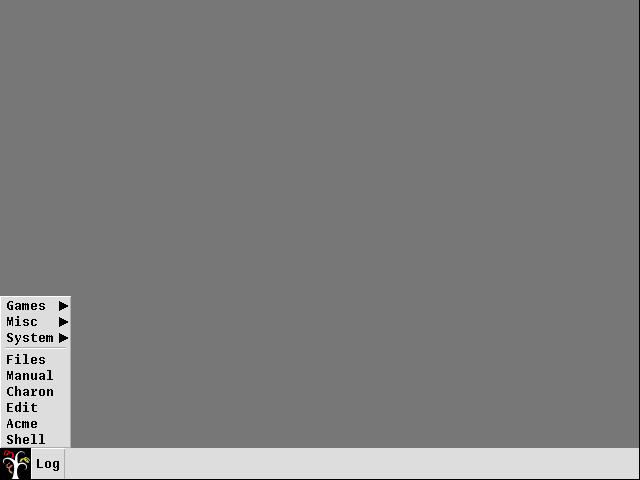
\includegraphics[width=0.5\textwidth]{start_menu.png}
      \caption{Inferno's window manager with start menu}
    \end{wrapfigure}

    For indeed it seems what have stridden upon a system wholly encompassed by the colour of despair with no task to accomplish but to gaze upon its grey insipidness. You should not fret, though, for this is but a disguise; hiding beneath its ghastly appearance lie programs who are waiting eagerly to be used. To aid you in your journey, you shall henceforth be provided with photographs of the system as I see it, since I believe this will simplify your journey considerably; indeed, those poor souls whom the ability to use Inferno has not been bestowed for they lack a proper system install it onto, are what these photographs will aid most substantially, as they may therefore see the happenings of our doings without needing their own installation.

    But withal, those keenly-eyed amongst us may have observed the rather small square icon at the very bottom left of the screen whose appearance is reminiscent of that of a tree which is situated next to a sickly grey box containing the text ``Log''. The latter's function should be quickly understood by even the more simple-minded — it opens a window containing logs, which tell us about things that have inevitably gone wrong — and the function of the tree-like one, too, should be easily understood; for what hides in this precise spot on most operating sytem? Why indeed, it is the start menu whose function, in most systems, encompasses the display of programs to start.

    Even its appearance is rather colourless and uninspiring, for it consists merely of three sub-menus and six readily executable programs — of which there is one titled ``Manual'' and that shall be the one we will inspect first, as it may prove invaluable to receive some additional information.

    \begin{wrapfigure}{R}{0.55\textwidth}
      \centering
      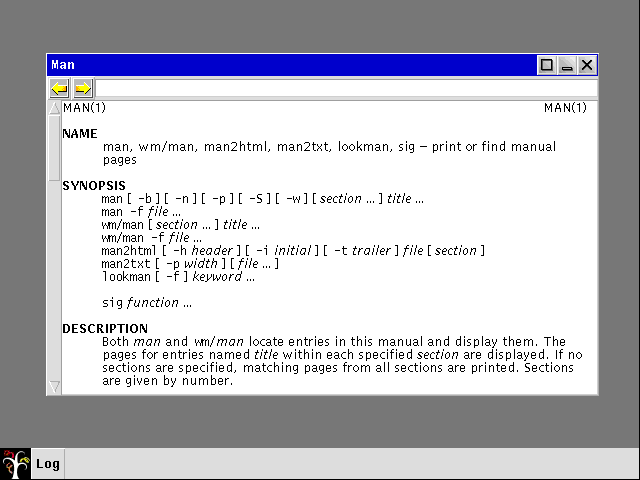
\includegraphics[width=0.5\textwidth]{manual.png}
      \caption{Manual}
    \end{wrapfigure}

    What then appears is a window filled with text — as one would expect a manual to be — and a search bar across the top; this can be used to investigate a particular command's or program's function. Thus, if we wished to be presented with information regarding the window manager, simply typing \texttt{wm} into its search and pressing the \textit{Enter} key will yield said requested information.

    This program will prove itself invaluable, for it will dispense information regarding practically every single part of this operating system and we shall be referring back to it frequently.

    Time has now come to open pandora's box and examine what programs Inferno provides for us, how they are used and what can be done with them. \newpage

    \chapter*{Combing through Hell's Inventory}
      \markboth{Combing through Hell's Inventory}{Combing through Hell's inventory}
      \addcontentsline{toc}{chapter}{Combing through Hell's Inventory}

    \epigraph{``O how unlike the place from whence they fell!''}{\textit{John Milton\\Paradise Lost, Book I}}

    Upon having finally entered and briefly explored Inferno, we shall now begin our more thorough investigations of which kinds of utensils are available to us of which there appear to be numerous. In the following section we shall explore these in brief, for most of them are meagerly equipped with functions; yet there do exist a few that are able to do much and we shall thus look at these in more detail.

    I also provide you with photographs of these programs frequently.

    \section*{Files}
      \markboth{Files}{Files}
      \addcontentsline{toc}{section}{Files}

    Its name is, I believe, rather self-explanatory — it merely provides us with a list of files; yet, it appears to struggle doing so, for when one tries to open it, one is pestered by the log, which puts itself into the spotlight to warn us of missing items. Lamentably, its messages are of little help; they speak of the user \texttt{root} which, apparently, does not exist; and they also speak of a missing \textit{plumber} — truly tragic that the system seems to be having problems with its plumbing.

    \begin{wrapfigure}{R}{0.55\textwidth}
      \centering
      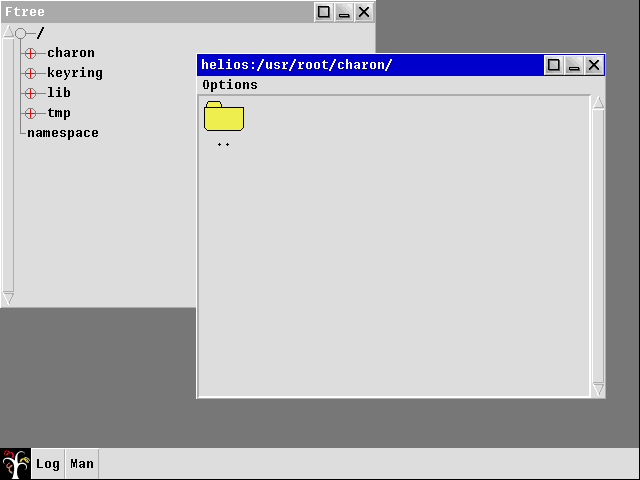
\includegraphics[width=0.5\textwidth]{files.png}
      \caption{Inferno's \textit{Files} program}
    \end{wrapfigure}

    However, I believe our newly acquired friend, the \textit{manual} may be of help; let us thus spawn it hither once more and ask it for advice. It tells us the following: —

    \begin{quote}
      Plumber provides high-level message-passing between applications.
    \end{quote}

    This helps us discern what its purpose is; but alas, this helps us but scantly in ascertaining what the error is implying — indeed it appears our installation is missing this plumber altogether, but what is one to do to mitigate this?

    \begin{wrapfigure}{R}{0.55\textwidth}
      \centering
      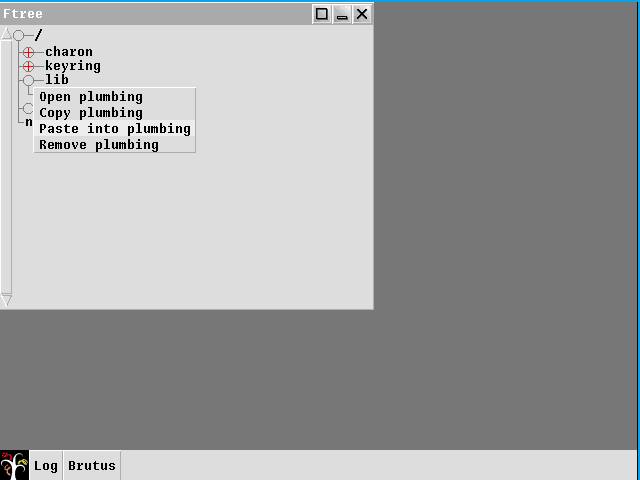
\includegraphics[width=0.5\textwidth]{files-menu.png}
      \caption{Inferno's \textit{Files} program with menu}
    \end{wrapfigure}

    In addition to the aforementioned information — and more, for I showed but the main definition of what plumber does —, the manual page provides us with a file path wherein we are to find its rules for a specific user: \texttt{/usr/user/lib/plu-\\mbing}, wherein \texttt{user} must be replaced by the user who is currently using the sytem.

    Upon entering the \texttt{/usr} directory, one immediately notices that there is but one lonely user present, namely \texttt{inferno} and the prioly mentioned \texttt{root} user is nowhere to be found.

    This discovery lead me to believe that a root user must be created, a task that, due to Inferno's philosophy of all things being files, should be easily accomplished by simply copying the \texttt{inferno} folder and renaming it \texttt{root}; hence we created a second user, the one which Files was so desparately longing after, whereupon we should have finally gained the ability to execute the File program without it deeming it necessary to throw errors at us for things we did not do.

    Indeed, having done so appears to have tempered him who dwells below the surface of Inferno, for Files opens without errors; why, it finally allows us to click folders to open them at inspect their contents freely and without being disturbed.

    But withal, one may now ask oneself, has what I have just done really been the correct way? Surely, one should be able to log in as a different user; yet, unfortunately, I have been unable to ascertain how that is possible, for the manual page of \texttt{wm} proved to be of but meager help. There seems to exist a command titled \texttt{logon} which, if used with \texttt{wm}, is supposed to provide a screen whereon a user can login; but alas, I have been unable to get it working.

    \begin{wrapfigure}{R}{0.55\textwidth}
      \centering
      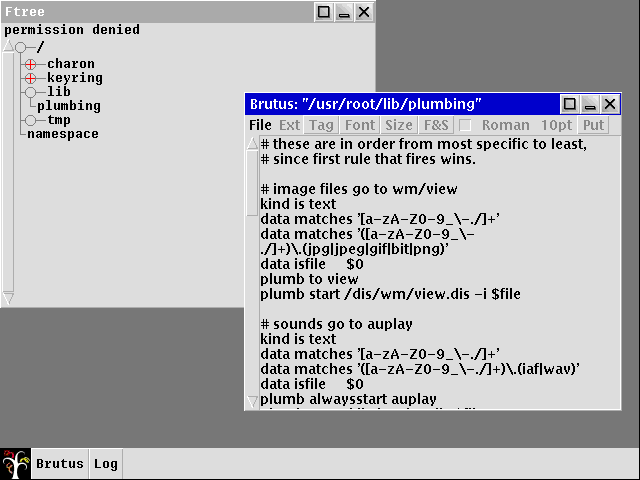
\includegraphics[width=0.5\textwidth]{brutus.png}
      \caption{Brutus}
    \end{wrapfigure}

    Upon having fixed this program, one is now able to open, copy or remove files by clicking and pressing the left mouse button; thereupon, a menu appears where one may select an option. Should you choose the option to open a particular file, a new program will reveal itself titled \texttt{Brutus}; yet mysteriously, one is unable to find it inside the start menu, for there it is nowhere to be found — an elusive program indeed, and one that, I must admit, I trust but little; for it appears to have gotten its name from one of those vile politicians who, back in yonder days of the Roman Empire's glorious rule, stabbed Gaius Julius Caesar to death; why indeed, it was he whom Caesar asked, ``Et tu, Brute?'' in Shakespeare's play for Caesar did not believe even Brutus would have betrayed him; and as I have learnt to not trust this name, I shall be weary of it here, too.
    
    Yet we are lucky, for there exists a manual page regarding \texttt{Brutus} which proclaims that: —

    \begin{quote}
      Brutus is a multi-file editor for UTF format text files.
    \end{quote}

    Indeed, it appears to be but a mere text editor wherewith one is able to edit and view files; yet this raises two questions, for why can it not be found within the start menu and what is the reason for the existance of two text editors? Since, apart from vicious Brutus, there is another; one which is much more simple, something reflected in its name too, for it is called — in a truly uncreative Unix-fashion — merely \textit{Edit}. I wonder, whither has their philsophy been tossed; their philosophy of being minmalist, for I cannot grasp the existence of two editors — whereof one being notably inferior — whose functions and purposes are nigh identical.

      \section*{Charon}
        \markboth{Charon}{Charon}
        \addcontentsline{toc}{section}{Charon}

      \begin{wrapfigure}{R}{0.55\textwidth}
        \centering
        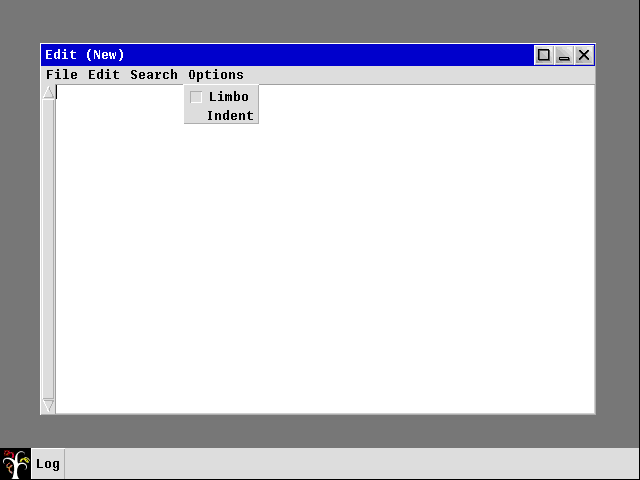
\includegraphics[width=0.5\textwidth]{edit.png}
        \caption{Edit and its options menu}
      \end{wrapfigure}

      Continuing Inferno's horrid tendency of naming its programs after beings whose names shall forever be associated with Death, its web browser is titled \texttt{Charon}; indeed he, from whom this program has received its name, is the ferryman of Hades; he whom the Greeks believe one must pay a toll for otherwise they mayn't cross the river; the river Styx; the infernal waters, which separate the land of those who live and those who are dead; and he who is unable to pay his dues is forced to wander its shores for aeons before Charon shall return to take him to yonder side. Indeed, it was the custom of the Greeks and the Romans to place a coin into the mouths of the Dead, lest they arrive at the shores of the sulphurous waters, impoverished and without a coin to part with whereupon they would be damned to wander its dismal coasts for years upon years, for Charon would not take aboard those poor souls who did not pay; nay, he would leave them ashore.

      Truly, it appears that even we have been left ashore, damned to wander aimlessly, for we are unable to open websites but the one of Inferno itself. Must we, too, wait aeons for him to return to us so that he may row us across the Internet river at speeds unfathomable, to allow us to reach other computers, located half-way across the world, in but the blink of an eye?


      It surely appears to be the case, for I have been unable to ascertain its problem. It complains of a missing \texttt{host} file, but the lack of verbosity is truly aggravating; and lest my computer gets thrown through the window I shall continue with the next program.

      \section*{Edit}
        \markboth{Edit}{Edit}
        \addcontentsline{toc}{section}{Edit}


      Having briefly touched upon the subject of editors when discussing Files and the editor wherewith it comes bundled, Brutus, which it opens when attempting to view files, we shall one more comment on the subject of editors. Since, as we have observed, one cannot spawn Brutus from the start menu; nay, for there one may find but plain \textit{Edit}, a truly bleak program, wholly overshadowed by its seemingly big brother Brutus. Its option menu sparsely populated and its contents cryptic — for what is \textit{Limbo}?

      I must confess that I indeed do know of Limbo and its purpose; for it is the language wherein one is supposed to write programs for Inferno, to extent its reach into the world and to expand upon its existing functions. But alas, 'tis a subject much too advanced for us at this stage, for barely do we even know Inferno's core functions; how are we, then, to write programs for it? Fear not of missing out, for we shall examine Limbo, but first we must understand Inferno's inner works; only having done thusly shall we be aptly qualified to use Limbo.

      Yon program, which reminds one of those used in bygone days, truly appears to be but a meager editor and whereof not much can be said — it does, indeed, enable one to edit files, but this is all it is able to accomplish.

      \section*{Acme}
        \markboth{Acme}{Acme}
        \addcontentsline{toc}{section}{Acme}

      For once we are presented with a program whose name is rather descriptive; for it derives from the Greek's \textit{$\alpha$$\kappa$$\mu$$\eta$} which one can translate into English as \textit{zenith} and truly, it is the most advanced of all programs we have thus far seen; and despite its appearance — which, alas, departs but little from that of Edit or Brutus —, it appears to be the system's peak. Indeed, it strikes one as being feature-rich — that is, in Inferno's terms, for the majority of its programs are rather barren — and rather sophisticated. Therefore, I thought it pertinent to engage with it more thoroughly and that we shall do.


      \begin{wrapfigure}{R}{0.55\textwidth}
        \centering
        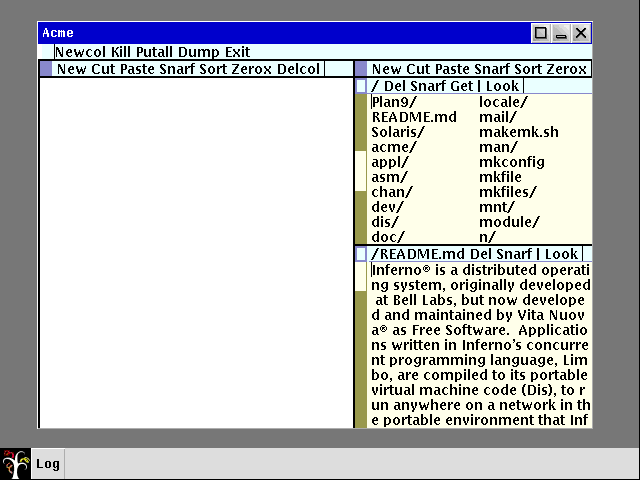
\includegraphics[width=0.5\textwidth]{acme.png}
        \caption{Acme}
      \end{wrapfigure}

      I was initially confused wherefore the name \textit{Acme} had been chosen, for I believed it to be but a mere acronym; yet this appears not to be the case and I believe my judgment of its name having been chosen for its omnipotence, as I believe one can do but little with Inferno were it not for Acme, is to be deemed accurate. Perhaps, though, I exaggerate, but I am confident in believing that most tasks would require one to do a much larger amount of work without it.

      Ostensibly, one may wonder for what purpose the other programs have been constructed, since, indeed, Acme does what all other programs mentioned thus far — with the exception of Charon — can. The manual page for Acme describes it thusly: —

      \begin{quote}
          Acme manages windows of text that may be edited interactively or by external programs. The interactive interface uses the keyboard and mouse; external programs use a set of files served by acme[.] [...]
     \end{quote}

     Speaking of its manual page, it is the largest I have seen thus far, containing a great deal of information regarding its functions. Therefore, it shall be impossible for us to cover all its parts in-depth — indeed, we shall leave out a fair portion of it — and instead we shall be focussing on a small number of things I deem to be imporant or of interest.

     The first aspect of this program I wish to illustrate is its mouse support; for, indeed, it may be controlled by one's mouse, yet its controls may seem rather unintuitive to those more accustomed to modern systems. One must also be prudent to differentiate between the title bar Acme has been imparted with by \textit{wm} and its inner title bars, as the one which it has receieved from \textit{wm} controls but the ``outer'' window of Acme itself; that is, it controls all of Acme, but not less and the inner parts of Acme cannot be manipulated or controlled using the outer title bar. The outer title bar, should my explanation sound too bizarre, is the title bar which contains the name of the program on its left side; and three buttons which enlarge, minimise or close the window respectively on the right side.

     These two title bars have two rather distinct functions and controls, for the outer title bar is controlled in a fashion similar to that which is used on operating systems such as \textit{Windows} wherein you are required to push the left mouse button to activate their functions. Yet the inner title bars depart from this control scheme quite significantly — and wherefore this has been done eludes me greatly —, for one is required to make is of all available mouse buttons; indeed, using the middle mouse button is a frequent occurence in Inferno.

     I belive it pertinent, though, to commence by studying the individual parts of the inner title bars prior to my explanation of their controls — for how may one control something one knows but little knowledge of?

    As visible on the provided photograph, there exist several windows within Acme, whereof each is in the possession of its own bar; yet there also exists a title may I shall henceforth call the \textit{master title bar}, for therewith one may control all of the inner windows — indeed, one may spawn a new inner window with it. Peculiarly, there appears to exist an \textit {Exit} field on the master title bar, rendering the \textit{X} of the outer title bar redundant; surely, leaving it out would have not impeded the program's functionality in any way but could have aided in making it appear less complicated.

    In addition to this absolutely expendable button and the aforementioned button permitting one to spawn a new column — or inner window —, three other buttons can be observed; namely \textit{Kill}, \textit{Putall} and \textit{Dump} — truly abhorrent names, I must confess, and ones that do not appear to have any discernable function, for clicking them seems to do but little. Thus, consulting the manual would no doubt be advantageous. 

    Upon having done so, one should have ascertained that \textit{Dump} saves Acme's current state — which, I believe, encompasses the currently opened inner windows / column and their position within Acme itself — to ``acme dump''; it truly appears these names have been chosen by someone of but little good taste, for they are quite dismal beyond any doubt — surely, the choosing of a less vulgar and perhaps more descriptive name would not have been too difficult a task.

    The function of the \textit{Kill} button is, to me, rather equivocal, for the manual has but little information regarding its function and merely states the following: –

    \begin{quote}
      ``Send a kill note to acme — initiated commands named as arguments''
    \end{quote}

    Given this rather tenuous explanation of its function is, unfortunately, insufficient for me to comprehend it; due to that, I shall refrain from commenting on it further and proceed with the last item, namely \textit{Putall}.

    Yet, I was forced to uncover, it, too, appears to have a rather cryptic manual entry, for it describes its function thusly: —

    \begin{quote}
      ``Write all dirty windows whose names indicate existing regular files''
    \end{quote}

    It is truly remarkable how a manual page has the ability to baffle one so greatly that he is thence even more perplexed as he was prior to having read it. For, indeed, why would there be dirty windows on an operating system; something that does not physically exist? Let us therefore continue by examining the other windows' title bars, even though they, too, appear to contain names I find much too cryptic.

    The very first item thereon is a simple square, either suffused entirely by a cerulean colour or merely posessing borders of that colour, in which case the other parts of the square are entirely white; yet the reason wherefore there exist two distinct types of rectangles escapes me, for they seem to fulfill the exact same functions, namely moving the window around. Indeed, if one wishes to change the location of one of Acme's inner windows, one is required to press and hold the left mouse button and hence move the window whither one desires. 

    Located to its right, a button titled \textit{New} can be found, wherewith one may spawn additional inner windows.

    Thereafter appears \textit{Cut}, which allows one to remove the text which has been selected and, as the manual states, which the computer then places into the ``snarf buffer'' — horrid naming conventions will, undoubtedly, not disappear henceforth. \textit{Snarf} appears to be the name of the system's clipboard, which also explains the function of the \textit{Snarf} button which can be seen further to the right — it copies selected text into the clipboard.

    \textit{Zerox} has a rather intriguing function, for upon having clicked it, a new windows containing the text we had previously selected, emerges. 

\end{document}
